\documentclass[a4paper,10pt,fleqn]{article} % Definiert Papier = A4;
%                                            % Schriftgrösse = 10Punkte;
%                                            % Mathe.-Gl. Modus = linksbündig
%                                            % (siehe http://lefti.amigager.de/latex/Aufbau.html)
%
\usepackage{../common/layout}
\setcounter{tocdepth}{4}   %= Aufnahme in das Inhaltsverzeichnis *
\setcounter{secnumdepth}{4}  % = Nummerierung vertiefen *

\newboolean{STANDALONE}
\setboolean{STANDALONE}{false}

\newboolean{EMBED}
\setboolean{EMBED}{false}

\newboolean{DC}
\setboolean{DC}{false}

\newboolean{BLDC}
\setboolean{BLDC}{false}

\newboolean{STEPPER}
\setboolean{STEPPER}{false}

\newcommand{\BLDCPath}{src/bldc}
\newcommand{\DCPath}{src/dc}
\newcommand{\STEPPERPath}{src/stepper}

\newcommand{\BIBLIOGRAPHY}{src/common/et-gruppe_source}

\newcommand{\EtPath}{Enddokumentation/ET-Gruppe}

\newcommand{\myTitel}{Realisierung eines\\
autonomen Ballwerfers}
\newcommand{\myDokumentTyp}{Anhangsdokument}
\setboolean{STANDALONE}{false}
\setboolean{EMBED}{true}
\setlength{\parindent}{0em} 
\begin{document}
    %
    % Deck- und Titelblatt
    %
    \begin{titlepage}
    \begin{center}
        \parindent0pt{\Huge\bfseries \myDokumentTyp}\\[0.5cm]
        {\huge PREN 1, Team 32}\\[1cm]
        Yves Studer\\
        Thomas Wiss\\
        Livio Kunz\\
        Niklaus Manser\\
        Matteo Trachsel\\
        Roger Gisler\\
        Pascal Roth\\
        \vspace*{1cm}
        {\Huge \myTitel}\\[0.5cm]
%        \begin{figure*}[h!]
%            \centering
%            
\includegraphics[width=0.7\textwidth]{Enddokumentation/Titelbild.JPG}
%        \end{figure*}
        
        \vfill{}
        {\normalsize Hochschule Luzern - Technik \& Architektur\\
         PREN 1}\\[0.6cm]
        {\normalsize Horw, Hochschule Luzern - T\&A, \today}
    \end{center}
\end{titlepage}

    \begin{titlepage}
    \begin{center}
        \parindent0pt{\Huge\bfseries \myDokumentTyp}\\[0.5cm]
		{\huge PREN 2, Team 32}\\[2em]
        \begin{tabular}{ll}
            Yves Studer                & Thomas Wiss \\
            Dorfstrasse 28             & Bachhüsliweg 4a \\
            6264 Pfaffnau              & 6042 Dietwil \\
            +41 79 705 48 88           & +41 79 604 93 61 \\
            yves.studer@stud.hslu.ch   & thomas.wiss@stud.hslu.ch \\
                                       & \\
            Livio Kunz                 & Niklaus Manser \\
            Hubelmatt 7                & Brunnmattstrasse 11\\
            6206 Neuenkirch            & 6010 Kriens \\
            +41 79 811 53 03           & +41 77 405 58 56 \\
            livio.kunz@stud.hslu.ch    & niklaus.manser@stud.hslu.ch \\
                                       & \\
            Matteo Trachsel			   & Roger Gisler \\
            Ogimatte 7                 & Eyrüti 16\\
            3713 Reichenbach           & 6467 Schattdorf\\
            +41 79 511 57 88           & +41 79 729 55 34 \\
            matteo.trachsel@stud.hslu.ch & roger.gisler@stud.hslu.ch \\
            						   & \\
            Pascal Roth			       & \\
            Dorfstrasse 18			   & \\
            6275 Ballwil		       & \\
            +41 79 717 68 94	       & \\
            pascal.roth@stud.hslu.ch   & \\
        \end{tabular}\\
        \vspace{3em}
        {\Huge \myTitel}\\[5em]
        Dozent: Markus Thalmann\\[2em]
        Hochschule Luzern - Technik \& Architektur\\   
        Interdisziplinäre Projektarbeit 2015
        \vfill{}
        Horw, Hochschule Luzern - T\&A, \today
    \end{center}
\end{titlepage}
    %
    % Inhaltsverzeichnis umbenennen und anschliessend einen Seitenumbruch
    %
    \renewcommand{\contentsname}{Inhalt}
    \tableofcontents
    \newpage 
    %
    % Start mit der eigentlicher Arbeit
    %    
   
	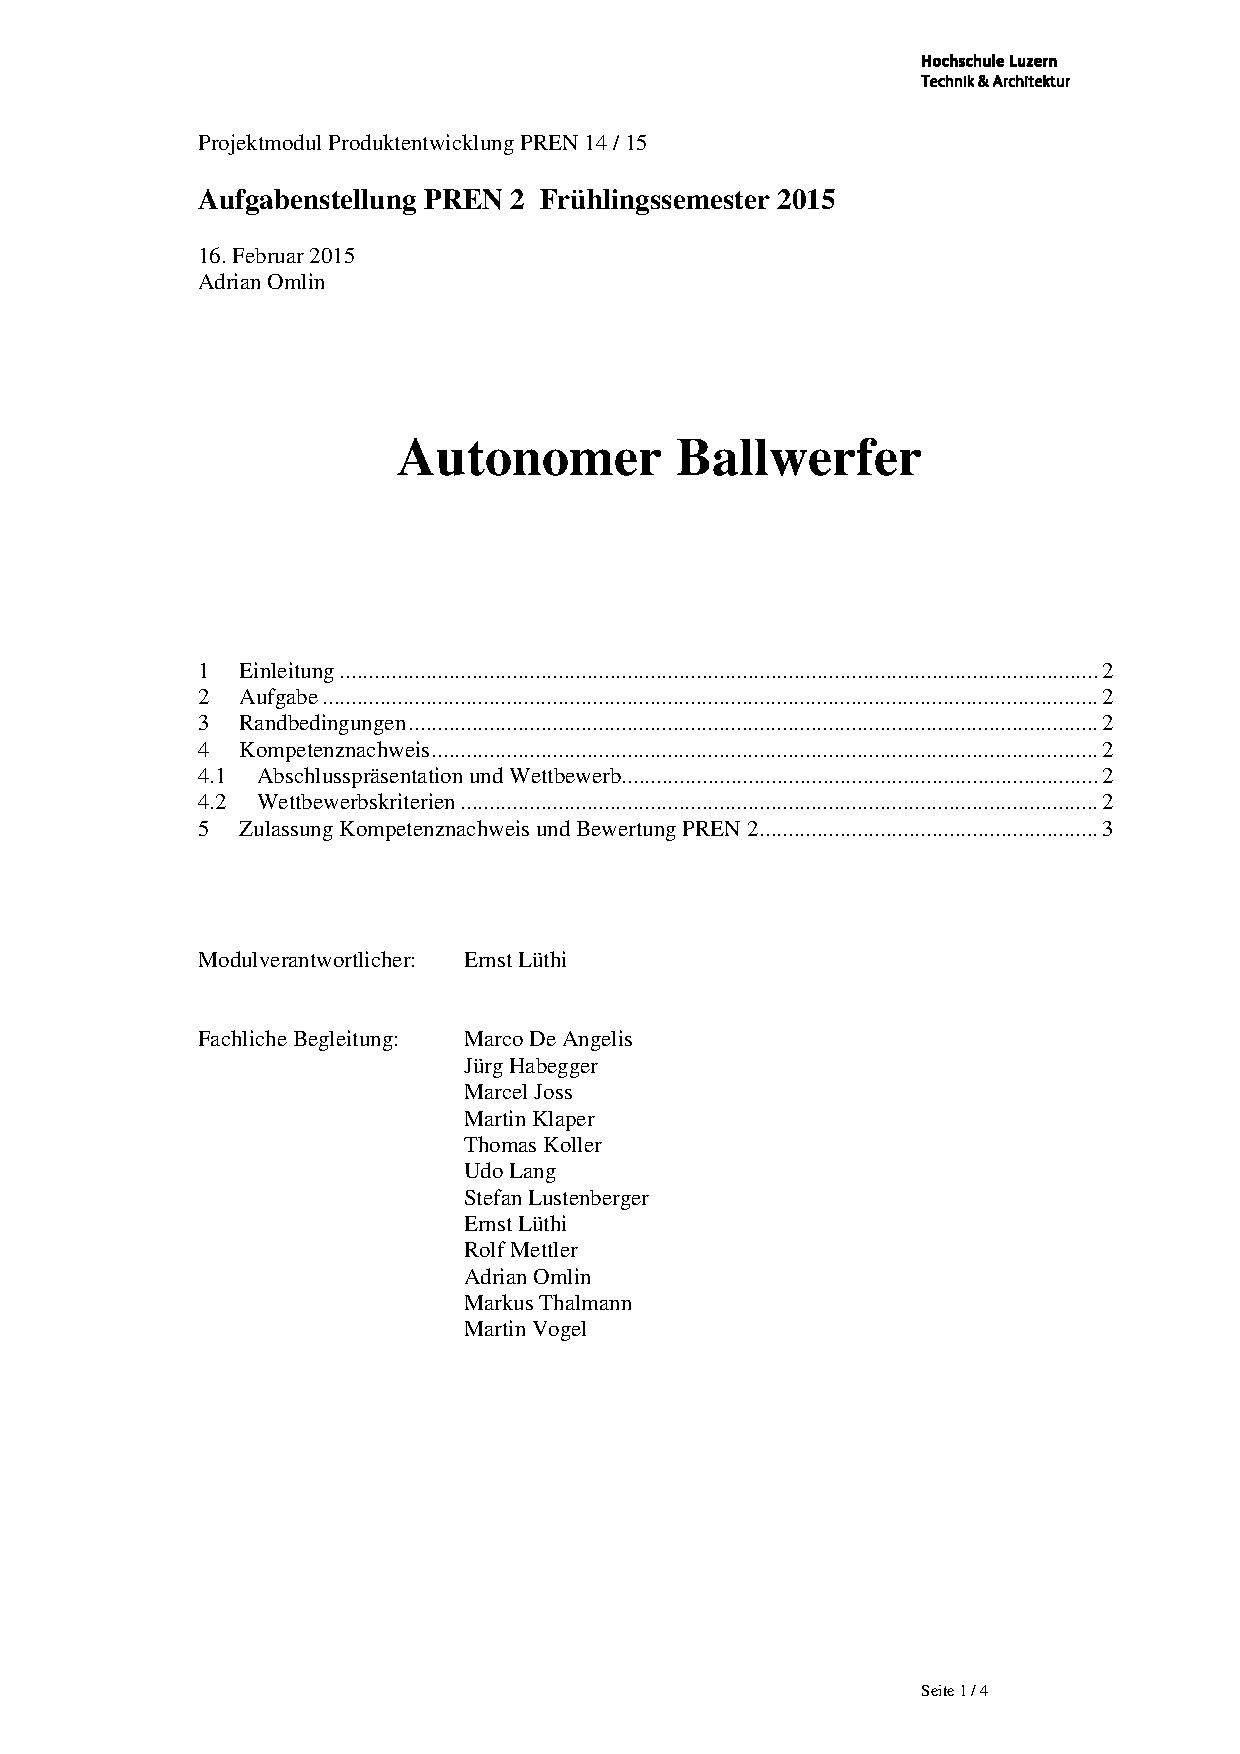
\includepdf[page=1 , offset=0cm -1.9cm, width=1.05\textwidth,picturecommand={\centering},pagecommand=\section{Aufgabenstellung PREN 2}{\thispagestyle{fancy}},]{Anhangsdokument/Aufgabenstellung_PREN2_F15.pdf}
	
	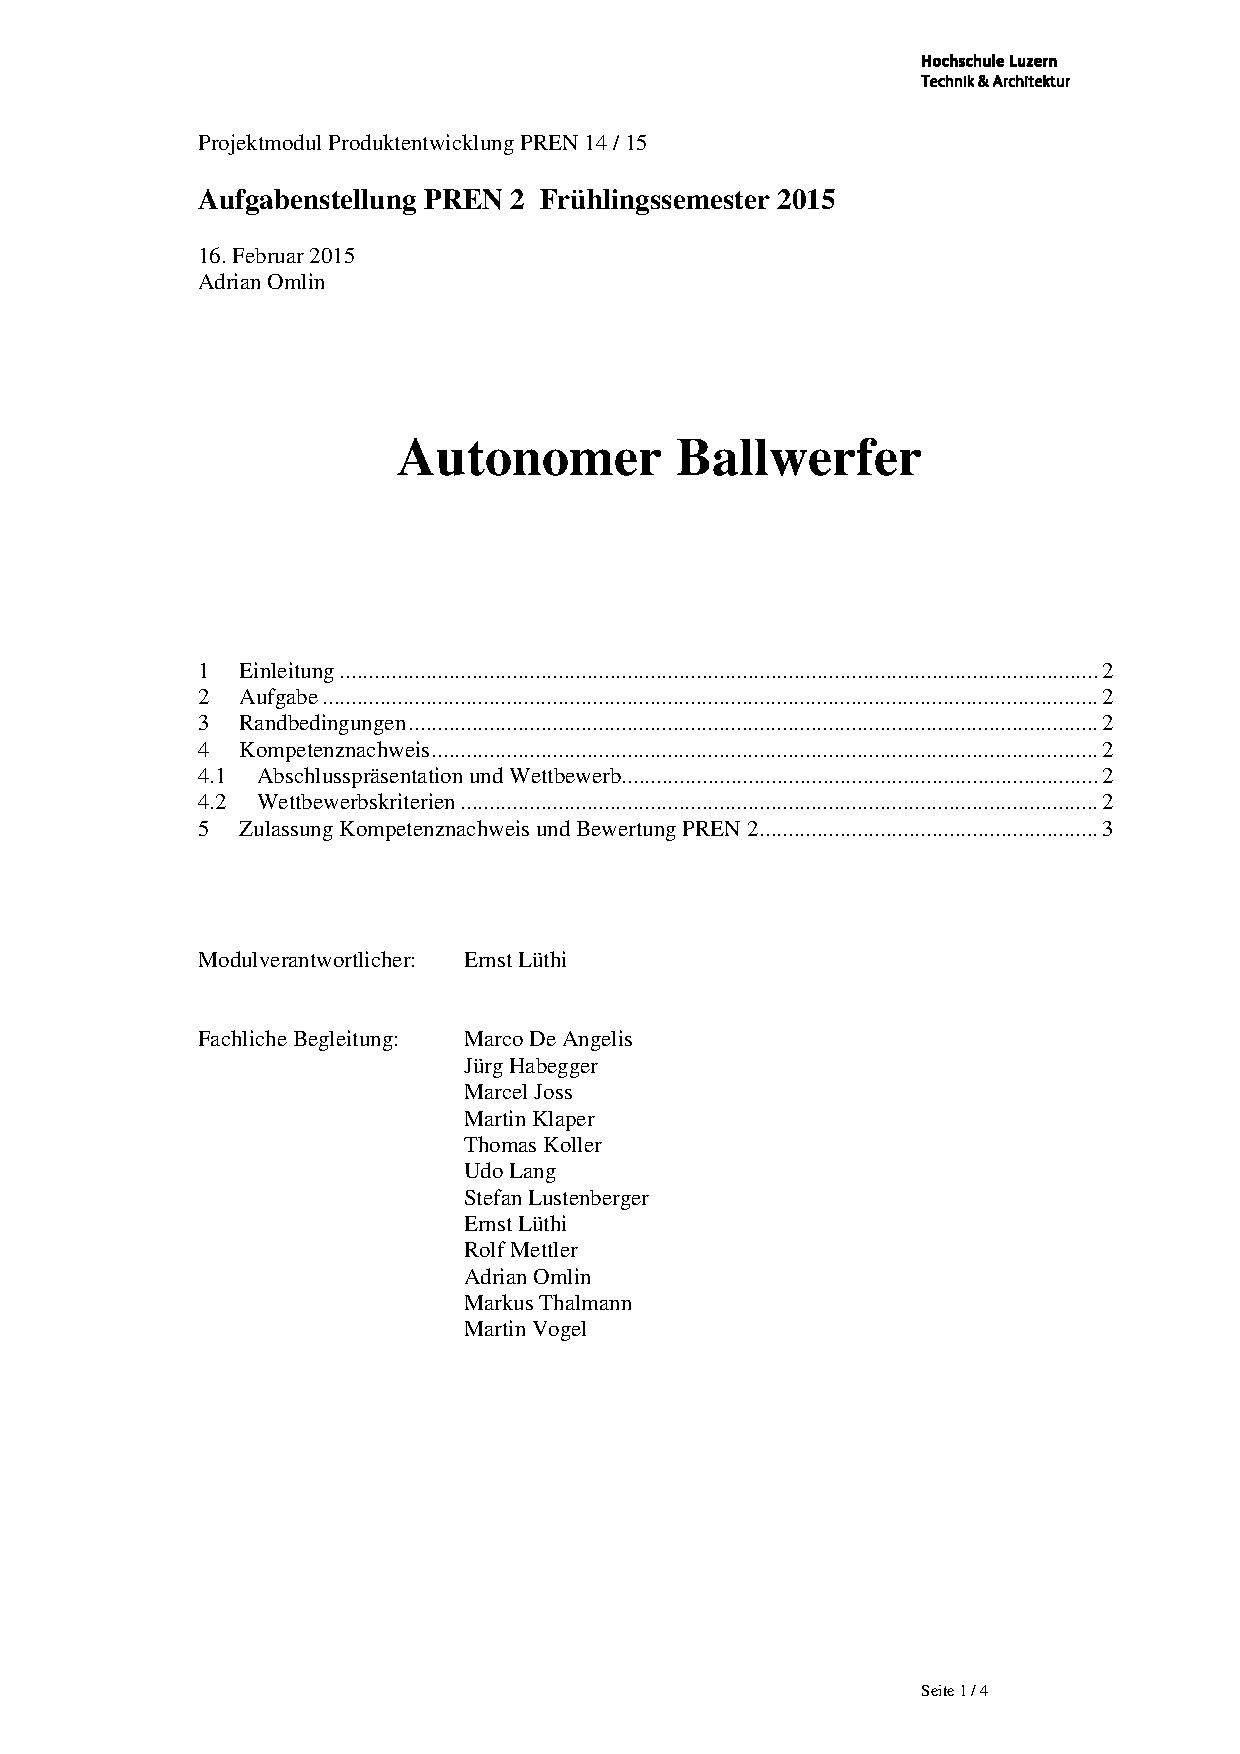
\includepdf[page=2- , offset=0cm -1.60cm, width=1.1\textwidth,picturecommand={\centering},pagecommand={\thispagestyle{fancy}},]{Anhangsdokument/Aufgabenstellung_PREN2_F15.pdf}
	
	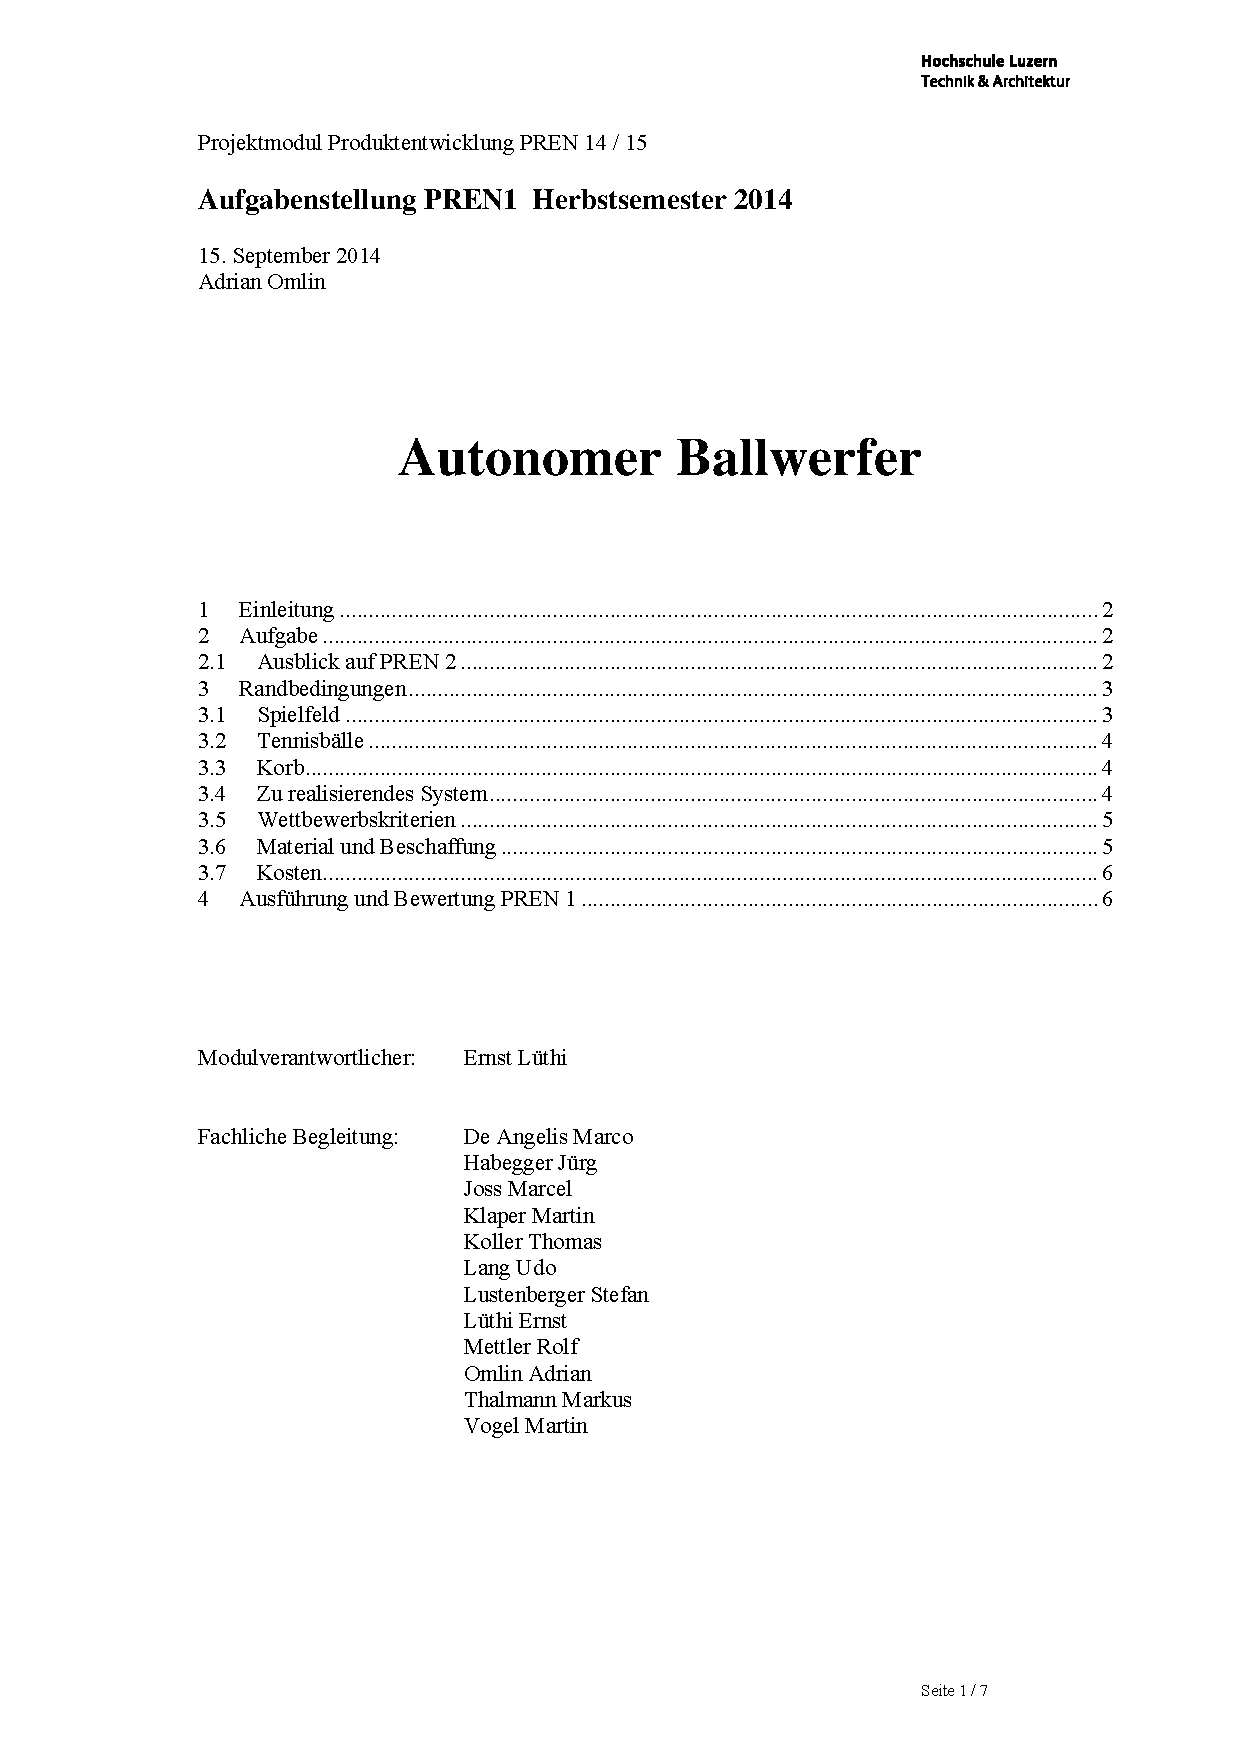
\includepdf[page=1 , offset=0cm -1.9cm, width=1.05\textwidth,picturecommand={\centering},pagecommand=\section{Aufgabenstellung PREN 1}{\thispagestyle{fancy}},]{Anhangsdokument/Aufgabenstellung_PREN1_H14.pdf}
		
	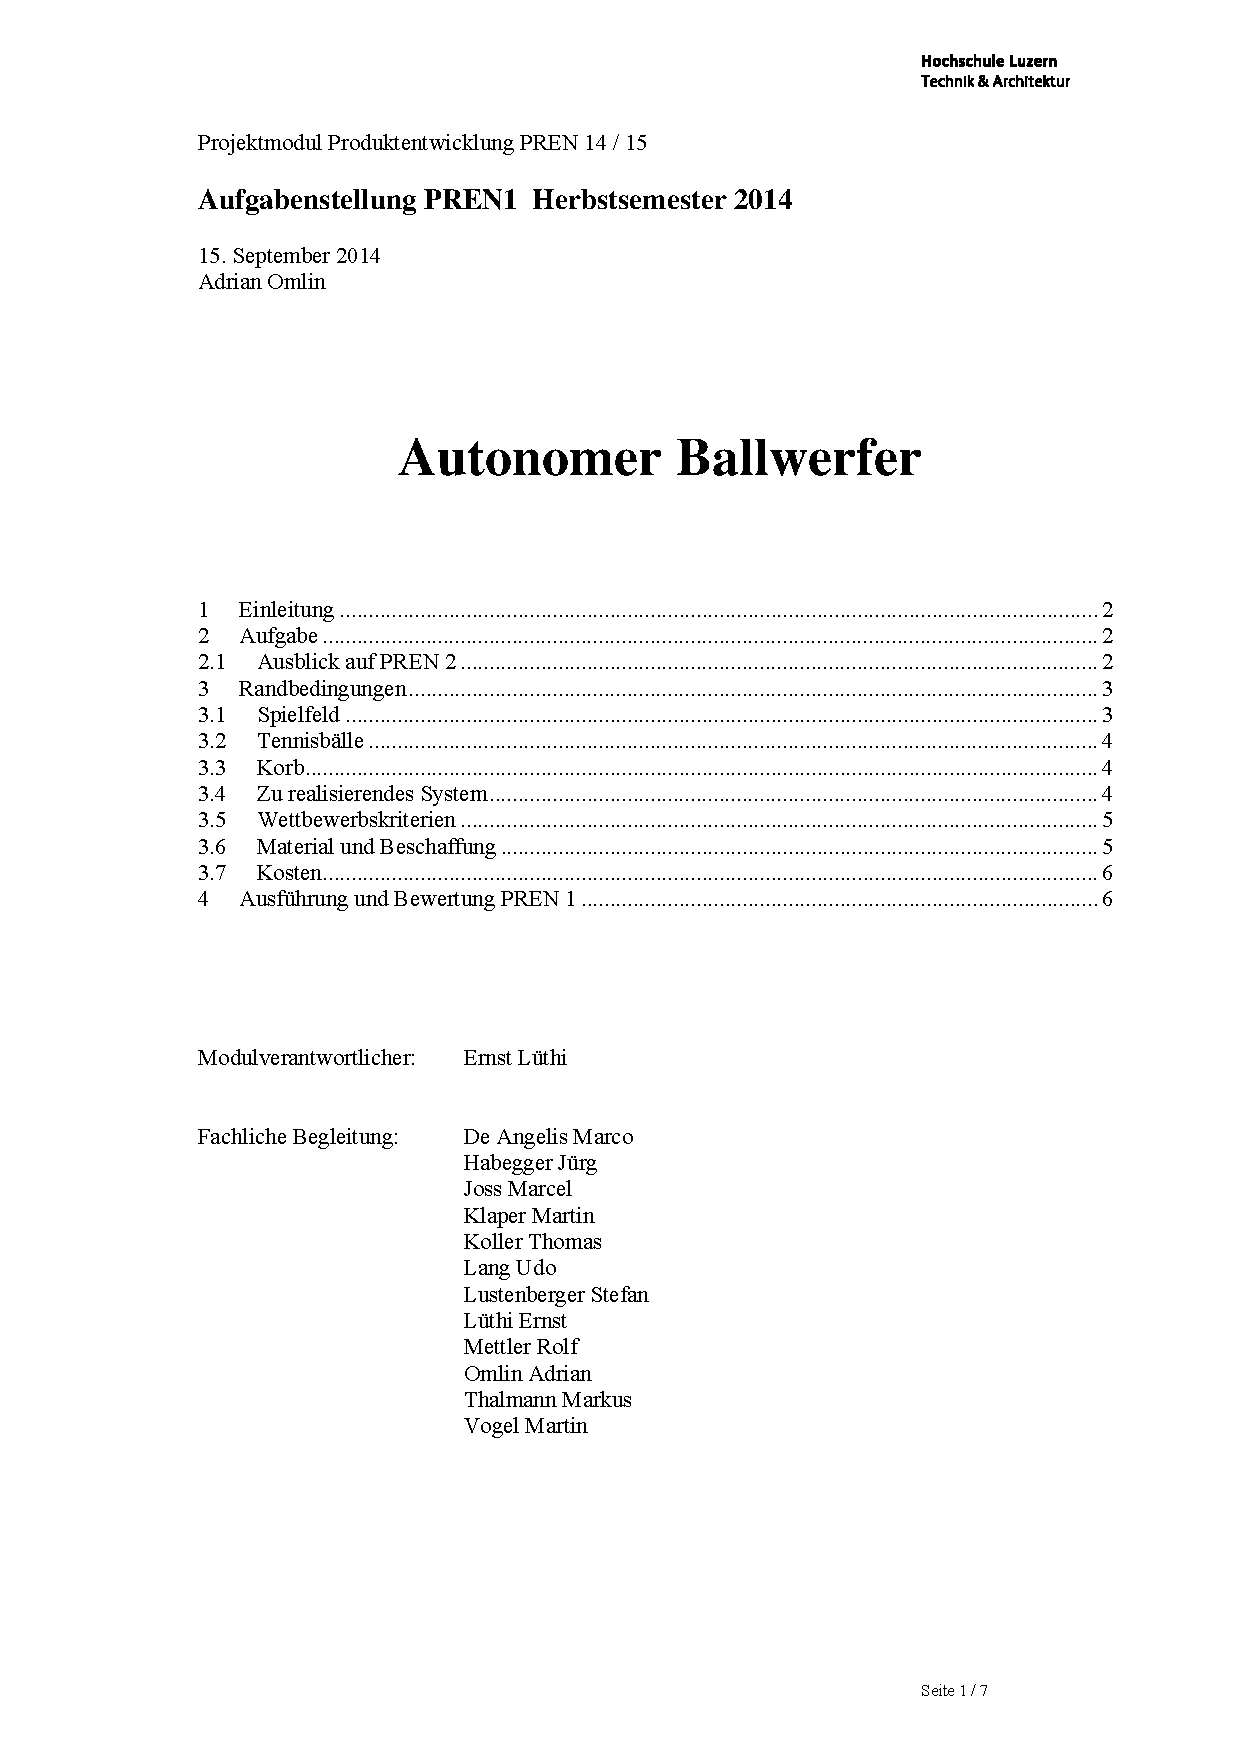
\includepdf[page=2- , offset=0cm -1.60cm, width=1.1\textwidth,picturecommand={\centering},pagecommand={\thispagestyle{fancy}},]{Anhangsdokument/Aufgabenstellung_PREN1_H14.pdf}
	
	\begin{landscape}
		\section{Risikokatalog}
		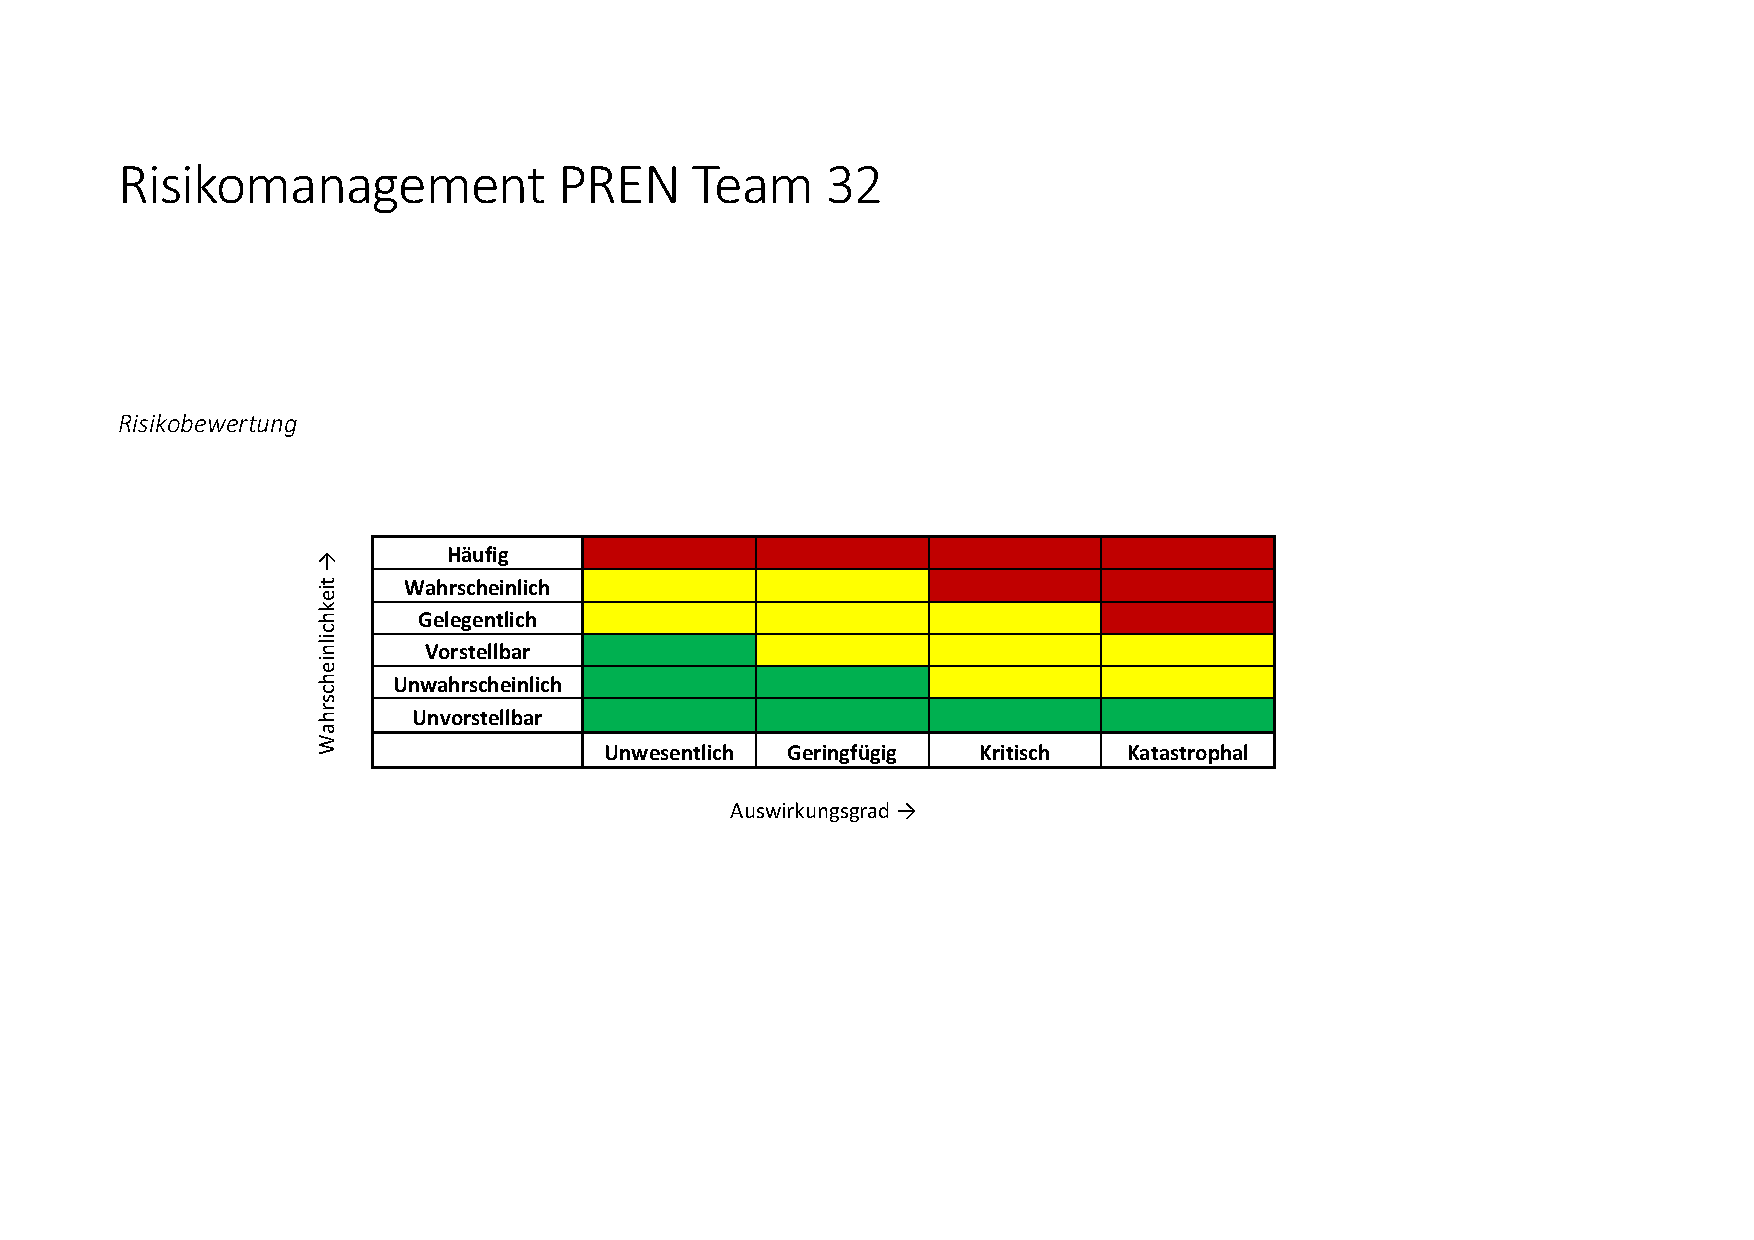
\includegraphics[page=1,scale=0.73,clip,trim=17mm 27mm 31mm 39mm]{Anhangsdokument/Risikomanagement.pdf}
		\newpage  			
		\includegraphics[page=2,scale=1,clip,trim=20mm 22mm 21mm 32mm]{Anhangsdokument/Risikomanagement.pdf}
		\newpage  			
		\includegraphics[page=3,scale=1,clip,trim=20mm 22mm 21mm 22mm]{Anhangsdokument/Risikomanagement.pdf}
		\newpage  			
		\includegraphics[page=4,scale=1,clip,trim=20mm 22mm 21mm 22mm]{Anhangsdokument/Risikomanagement.pdf}
		\newpage  			
		\includegraphics[page=5,scale=1,clip,trim=20mm 22mm 21mm 22mm]{Anhangsdokument/Risikomanagement.pdf}	
		\newpage  			
		\includegraphics[page=6,scale=1,clip,trim=20mm 22mm 21mm 22mm]{Anhangsdokument/Risikomanagement.pdf}	
	\end{landscape}  
\end{document}